




%\newpage
\section{Preprocessing} \label{sec:preprocessing}

We approach preprocessing in two steps. In the first step we prepare the dataset based on knowledge we obtained in \cref{sec:dataUnderstanding} and further analysis. 
Secondly, we transform the data with the help of various algorithms that are combined in a pipeline. 
%Secondly, we try many different approaches to transform the data, in instances where we can not be certain about the best method. \todo{der letzte halbsatz passt nicht}

\subsection{Data Preparation }
First, we implemented a custom loading function to put the four data sets into a usable format and harmonise known differences in encodings. In this step, the missing values marked $-9$ were replaced by \texttt{NaN} and the target variable was binarised by replacing all values greater than 1 by 1, as the UCI does not describe how the different positive cases (\textit{num} $\geq 1$) differ.

After that we removed irrelevant features such as IDs, dates, constants, undescribed columns as well as irrelevant columns according to the UCI. All of these columns are either not causally related to the presence of heart disease or cannot be examined for new patients because it is unknown what they measure. We also dropped the feature \textit{pncaden} because it is the sum of the binary variables  pain location, pain during exercise and relief on rest and therefore contains no additional information. 

After the removal 55 attributes remained and were used to train the first model. XGBoost was chosen for that because it natively can handle \texttt{NaN} values. The accuracy of a 10-fold cross validation without any tuning was 98,21. This result was unexpectedly good, which is why we analysed the importance of the different features. We found that the features belonging to the category of the \textit{Coronary angiograms} were serving as false predictors and therefore removed them, leaving us with 45 remaining features. To validate that the removal hat the desired effect the cross validation was run again this time with an accuracy of 76,50 and a more reasonable distribution in the weights of the features.   

After irrelevant columns were dropped the remaining features were analysed for inconsistencies. Here we found that \textit{thaltime} which describes the moment a measurement was taken during the exercise is sometimes larger than \textit{thaldur} which denotes the duration of the exercise. We replace \textit{thaltime} by \texttt{NaN} in all 17 instances in which this inconsistency was observed. Another inconsistency was found between the maximum heart rate (\textit{thalach}) and the heart rate at rest (\textit{thalrest}). If the maximum heart rate was below the resting heart rate the maximum heart rate was replaced by \texttt{NaN} since the values were unusually small.

\begin{figure}[h]
	\centering
	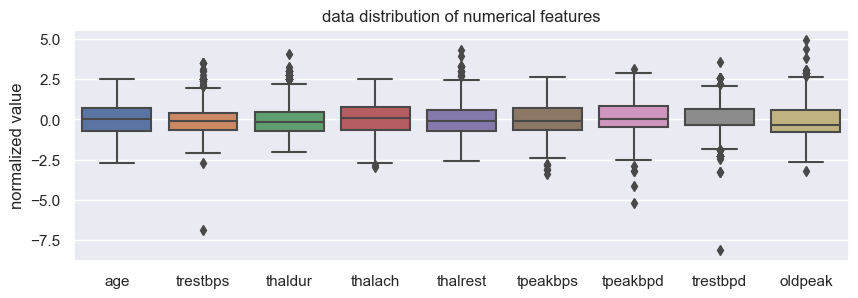
\includegraphics[width=\textwidth]{images/dataDistribution.png}
	\caption{data distribution of all numeric elements}
	\label{fig:dataDistribution}
\end{figure}
As shown in \cref{fig:dataDistribution} we created a normalised box plot of all numeric features to check for outliers. The features \textit{trestbps} and \textit{trestbpd} show extreme outliers with a value of 0. These are assumed to be incorrectly specified \texttt{NaN}s as stated in \cref{sec:dataUnderstanding} and are therefore replaced by \texttt{NaN}. All other outliers are not as extreme and come in groups. As the data contains sick persons, values diverging from the norm are expected. For these reasons we decided to keep these outliers as they might be a strong indication of a heart disease.

After handling all errors in the dataset the categorical features \textit{cp, restecg, slope, ca} and \textit{restwm} were oneHotEncoded and the remaining features were analysed regarding their pearson correlation. Only two pairs of features with substantive amount of data ($<$75\% \texttt{NaN}s) have a strong correlation ($>$75\%).  
These are asymptomatic chest pain $\leftrightarrow$ pain during exercise and \textit{rldv5} $\leftrightarrow$ \textit{rldv5e}. The first correlation seems plausible, as pain that only occurs under exercise is classified as asymptomatic. The features are still relevant, however, as the cases where there is no correlation are of particular interest. For \textit{rldv5} which denotes the height of the peak in the ECG during rest while \textit{rldv5e} is the same under exercise we are also interested in those cases where there is no correlation because this might be typically for people with a heart disease. In order to better understand the interrelationships two new features were computed two new features. Both represent the difference between a peak and a resting measurement. Once for the ECG ((\textit{rldv5\_diff})) and once for the blood pressure (\textit{thal\_diff}). 
Furthermore, we enrich the feature indicating whether a patient smokes by using the number of cigarettes per day and the length of time a patient has been smoking to infer the boolean variable. Hereby, the number of \texttt{NaN}s was reduced from 74\% to 43\%. 

\subsection{Hyperparameter Tuning} \label{subsec:hyperparametertuning}
Additionally to the hyperparamter tuning of the estimators, which is described in \cref{sec:datamining}, we also optimise the preprocessing steps by different hyperparameters.
%For hyperparameters and methods where we could not be certain, we try out multiple different combinations.\todo{liest sich doof}

Firstly, we added binning for the feature \textit{age}. We choose either 2 or 5 bins or no binning at all. We decided to use equal width binning due to the distribution of the age in the dataset. \todo{fand die erklärung vorher besser} The bins were encoded in an ordinal variable.

To impute the missing data we use a simple imputer. Missing values are replaced by the mean, median or mode of the feature. We decided against using a KNN imputer, because it is computationally much more expensive, while the iterative imputer is not used, as it is still experimental and therefore subject to change. Due to the high number of missing values and their uneven distribution across the features we decided to analyse how the number of imputed cells and number of features behave when columns with a certain amount of missing values are dropped. This is visualized in \cref{fig:percentageToBeDropped}.

\begin{figure}[h]
	\centering
	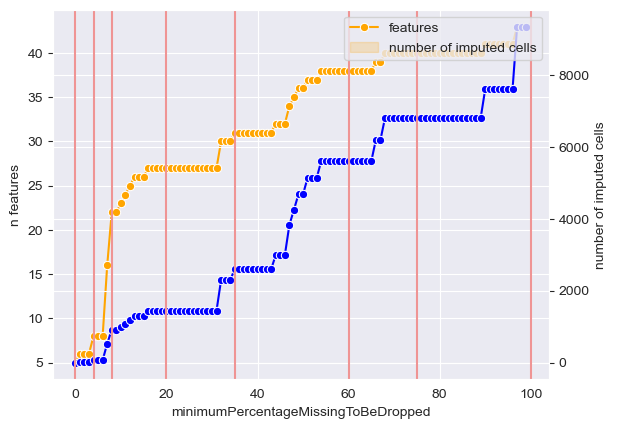
\includegraphics[width=\textwidth]{images/percentageToBeDropped.png}
	\caption{Number of features and values to be imputed by number of \texttt{NaN}s}
	\label{fig:percentageToBeDropped}
\end{figure}

It becomes apparent that there are certain steps where the number of features goes up a lot. To decide when a feature is included based on the number of missing values, we try the steps 0, 4, 8, 20, 35, 60, 75 and 100 \% in the model. They are shown as vertical lines in the graph. 

To account for the different ranges of the features different scalers are used. We only use scalers that are applicable for all features as some features contain negative values.
We compare the MaxAbsScaler, MinMaxScaler, PowerTransformer, RobustScaler, Standardscaler and Normalizer. As the hyperparameters of most scalers turn on or off core functionalities of the scaler, we decided to only tune the hyperparameter norm of the Normalizer with the norms l1, l2 and max.

To account for the slight imbalance of healthy and unhealthy patients we used oversampling and undersampling in the training data in comparison to no resampling. After this step the preprocessing is done. 


%The \textbf{MaxAbsScaler} scales the values of each feature by the maximum absolute value. Therefore, all values in [-1,1] can occur after scaling. \newline
%Using the \textbf{MinMaxScaler} results in values in [0,1] by shifting by the negative minimum and scaling by $maximum - minimum$\newline
%The values were normalized using the norms l1,l2 and max in the \textbf{Normalizer}. \newline
%The \textbf{PowerTransformer} alters the data to represent a gaußian like distribution. This is mostly used if heteroskedasticity occurs in the data. It was tried to fit the data to a standard normal distribution and without shifting and scaling by its mean and variance. \newline
%The \textbf{RobustScaler} was tried with and without scaling by the interquartile range and with and without shifting beforehand.\newline
%The \textbf{Standardscaler} was used with and without shifting by the mean and scaling by the standard deviation.\newline
%It was also tried, manly for comparison, to \textbf{passthrough} the values as they are.\newline